\documentclass[11pt,a4paper]{article}

\usepackage[utf8]{inputenc}
\usepackage[spanish,es-tabla]{babel}
\usepackage[margin=1.8cm,top=1.8cm,bottom=1.8cm]{geometry}
\usepackage{multirow}
\usepackage{colortbl}
\usepackage{xcolor}
\usepackage{longtable}
\usepackage{setspace}
\usepackage{graphicx}
\usepackage{array}
\usepackage{amsmath}
\usepackage{booktabs}
\usepackage{caption}
\usepackage{mathptmx}
\usepackage{hyperref}

% --- FONDO DE PANTALLA (MARCA DE AGUA) ---
\usepackage{background}

\backgroundsetup{
  contents={
\includegraphics[width=13cm,keepaspectratio]{logo-fondo.png}},
  opacity=0.08,
  scale=1,
  angle=0,
  placement=center
}
% -------------------------

\begin{document}

% =========================================================
% ENCABEZADO (CON LOGO SUPERIOR)
% =========================================================

\begin{center}
    
\includegraphics[width=2.8cm,keepaspectratio]{logo-fondo.png}\\[1ex]
    
    {\huge \textbf{UNIVERSIDAD ESTATAL AMAZÓNICA}}\\[1ex]
    {\large \textbf{Unidad de Organización Curricular:} \textcolor{gray}{Básica}} \hspace{1cm}
    {\large \textbf{Campo de Estudio:} \textcolor{gray}{Tronco común}}
\end{center}

\vspace{-0.2cm}

% =========================================================
% TABLA DE DATOS GENERALES
% =========================================================

\bgroup
\def\arraystretch{1.3}

\noindent
\begin{tabular}{|p{12.2cm}|p{4.2cm}|}
\hline

\rowcolor{green!15}
\multicolumn{2}{|>{\centering\arraybackslash}p{16.8cm}|}{
    \textbf{INFORME DE PRÁCTICAS DEL COMPONENTE PRÁCTICO-EXPERIMENTAL}
} \\

\hline

\multicolumn{2}{|l|}{
    \textbf{Nombre(s) del(de los) Estudiante(s):} Miguel Rodrigo Cahuasqui Hernández
} \\

\hline

\textbf{Asignatura:} Estructura de datos (UEA-L-UFB-032)
&
\multirow{4}{*}{\textbf{Calificación:}} 
\\

\cline{1-1}

\textbf{Fecha del informe:} 07 de Septiembre de 2026
& 
\\

\cline{1-1}

\textbf{Nº Práctica:} 03 (Semanas 9-10-11-12)
& 
\\

\cline{1-1}

\textbf{Título de la Práctica:} Guía de Prácticas \#03: Implementación de conjuntos y mapas
& 
\\

\hline

\end{tabular}

\vspace{-1.2pt}

% =========================================================
% CUERPO PRINCIPAL DEL INFORME (SIN ESPACIOS EN BLANCO)
% =========================================================

\noindent
\begin{longtable}{
    |>{\bfseries\centering\arraybackslash}p{3.2cm}|
    >{\setlength{\parindent}{0cm}\setstretch{1.12}}p{13.2cm}|
}

\hline
\endfirsthead

\hline
\endhead

\hline
\endfoot

\hline
\endlastfoot

% =========================================================
% INTRODUCCIÓN (INICIA DE INMEDIATO EN LA HOJA 1)
% =========================================================

Introducción
&
\textbf{1. Fundamentación Teórica y Justificación:}\newline
En el diseño y construcción de sistemas informáticos de alto rendimiento, la selección rigurosa de los Tipos Abstractos de Datos (TAD) es un factor determinante para garantizar escalabilidad, eficiencia computacional e integridad en la manipulación de información. La asignatura de Estructura de Datos profundiza en los mecanismos fundamentales para organizar y consultar colecciones con tiempos de respuesta óptimos (Cormen et al., 2022).

Las estructuras lineales convencionales (como listas contiguas o enlazadas) presentan un costo temporal de búsqueda y eliminación que escala linealmente $\mathcal{O}(n)$, obligando al procesador a iterar de manera exhaustiva elemento por elemento. Frente a este desafío, la teoría y aplicación de tablas hash permite la creación de \textbf{Conjuntos (\texttt{set})} y \textbf{Mapas o Diccionarios (\texttt{dict})}, los cuales logran un costo de acceso, inserción y verificación de pertenencia en tiempo constante amortizado $\mathcal{O}(1)$ (Goodrich et al., 2023; Weiss, 2021).
\\

\hline

&
\textbf{2. Marco Conceptual y Selección del Problema:}\newline
Un conjunto es una colección no ordenada de elementos únicos e inmutables (hasheables) que implementa operaciones algebraicas de la teoría de conjuntos: unión ($A \cup B$), intersección ($A \cap B$), diferencia ($A - B$), diferencia simétrica ($A \triangle B$) y verificación de subconjuntos ($X \subseteq A$). Por su parte, un mapa es una estructura asociativa que mapea una clave primaria única a un valor o registro de datos (Lutz, 2021).

En la presente práctica se selecciona el problema: \textbf{"Aplicación para el registro de jugadores y equipos en un torneo de fútbol"} (Torneo de Fútbol Amazónico UEA 2026), modelando la gestión integral de plantillas, auditoría de doble inscripción, control disciplinario y tabla de posiciones de clubes de la región amazónica ecuatoriana.
\\

\hline

% =========================================================
% DESARROLLO O PROCEDIMIENTO
% =========================================================

Desarrollo o procedimiento
&
\textbf{3. Escenarios y Actividades Desarrolladas:}\newline
Las actividades se ejecutaron en un ambiente de escritorio (computador personal con sistema operativo Linux, entorno Python 3.12 y control de versiones Git/GitHub CLI).

\textbf{3.1. Arquitectura Modular del Sistema:}\newline
Se diseñó una solución desacoplada en cuatro módulos principales:
\begin{itemize}
    \item \textbf{\texttt{models.py}:} Define las entidades \texttt{Jugador} (con clave primaria cédula hasheable), \texttt{Equipo} (con conjunto \texttt{jugadores\_ids}) y \texttt{Partido}.
    \item \textbf{\texttt{gestor\_torneo.py}:} Administra los mapas (\texttt{mapa\_equipos}, \texttt{mapa\_jugadores}) y los conjuntos universales y dinámicos (\texttt{conjunto\_todos\_jugadores}, \texttt{conjunto\_sancionados}).
    \item \textbf{\texttt{reporteria.py}:} Formatea y proyecta los datos en tablas visuales de terminal (tabla de posiciones, nóminas y auditorías).
    \item \textbf{\texttt{benchmark.py}:} Módulo científico que mide experimentalmente los tiempos de ejecución de listas vs. conjuntos y mapas.
\end{itemize}

\textbf{3.2. Implementación de Operaciones de Teoría de Conjuntos:}\newline
\begin{enumerate}
    \item \textbf{Diferencia ($A - B$):} Cálculo de jugadores habilitados para disputar una fecha deportiva mediante la sustracción de la nómina y los sancionados: $\text{Habilitados} = \text{Plantilla} - \text{Sancionados}$.
    \item \textbf{Intersección ($A \cap B$):} Auditoría automática de doble fichaje, verificando que la intersección de nóminas entre cualquier par de clubes sea vacía ($\emptyset$).
    \item \textbf{Unión ($A \cup B$):} Consolidación del padrón total de atletas participantes en un grupo regional sin duplicados.
    \item \textbf{Diferencia Simétrica ($A \triangle B$):} Comparativa analítica de futbolistas no compartidos entre dos instituciones.
    \item \textbf{Subconjunto ($X \subseteq A$):} Validación estricta de convocatorias y alineaciones previas al pitazo inicial, exigiendo que la nómina en cancha sea subconjunto de la oficial y disjunta con los sancionados.
\end{enumerate}
\\

\hline

&
\textbf{3.3. Declaración de Agente de Inteligencia Artificial:}\newline
Conforme a los lineamientos obligatorios de la guía docente:
\begin{itemize}
    \item \textbf{Agente de IA utilizado:} Google Antigravity (motorizado por Gemini 3.8 Flash).
    \item \textbf{Descripción del empleo:} Asistente de programación por pares utilizado para la estructuración arquitectónica del proyecto, diseño del benchmark comparativo Big-O, elaboración de la suite de 9 pruebas unitarias automatizadas y redacción técnica preliminar.
    \item \textbf{Porcentaje estimado:} 85\% asistencia del agente de IA en código base, algoritmos de benchmarking y pruebas; 15\% especificación contextual del problema amazónico, parametrización de reglas deportivas, depuración y validación por parte del estudiante Miguel Rodrigo Cahuasqui Hernández.
\end{itemize}
\\

\hline

% =========================================================
% RESULTADOS
% =========================================================

Resultados
&
\textbf{4. Resultados Obtenidos y Análisis de Rendimiento:}\newline

\textbf{4.1. Pruebas Unitarias Automatizadas:}\newline
Se ejecutó la suite completa de pruebas unitarias en \texttt{tests/test\_torneo.py}, validando el 100\% de las funcionalidades (9 pruebas ejecutadas y aprobadas en 0.005 segundos).

\textbf{4.2. Medición Experimental de Tiempos de Ejecución (Benchmarking):}\newline
Se evaluó el tiempo de búsqueda del operador \texttt{in} sobre colecciones sintéticas de diferentes tamaños $N$, promediando 500 iteraciones aleatorias:

\begin{center}
\small
\begin{tabular}{|r|r|r|r|r|}
\hline
\rowcolor{gray!20}
\textbf{N (Elementos)} & \textbf{Lista [$\mathcal{O}(n)$]} & \textbf{Conjunto [$\mathcal{O}(1)$]} & \textbf{Mapa [$\mathcal{O}(1)$]} & \textbf{Aceleración} \\
\hline
100 & 0.6926 $\mu$s & 0.0350 $\mu$s & 0.0303 $\mu$s & \textbf{19.8x} \\
1,000 & 5.7349 $\mu$s & 0.0433 $\mu$s & 0.0335 $\mu$s & \textbf{132.4x} \\
10,000 & 53.0618 $\mu$s & 0.1264 $\mu$s & 0.0878 $\mu$s & \textbf{419.9x} \\
100,000 & 741.4362 $\mu$s & 0.2311 $\mu$s & 0.2731 $\mu$s & \textbf{3,207.8x} \\
\hline
\end{tabular}
\end{center}

\textbf{4.3. Tiempos de Operaciones de Conjuntos ($N = 50,000$ elementos):}\newline
\begin{itemize}
    \item Unión ($A \cup B$): 7.24 ms
    \item Intersección ($A \cap B$): 5.44 ms
    \item Diferencia ($A - B$): 3.18 ms
    \item Diferencia Simétrica ($A \triangle B$): 3.50 ms
\end{itemize}

\textbf{4.4. Análisis de Ventajas y Desventajas:}\newline
\textbf{Ventajas:} Búsqueda instantánea $\mathcal{O}(1)$, garantía de unicidad sin comprobaciones manuales, sintaxis concisa y expresiva.\newline
\textbf{Desventajas:} Mayor consumo de memoria RAM debido al factor de carga de las tablas hash y obligatoriedad de que los elementos sean inmutables (hasheables).
\\

\hline

% =========================================================
% CONCLUSIONES Y RECOMENDACIONES
% =========================================================

Conclusiones y Recomendaciones
&
\textbf{5. Conclusiones:}\newline
1. La implementación de Conjuntos (\texttt{set}) y Mapas (\texttt{dict}) resolvió eficazmente las operaciones críticas de un torneo de fútbol, reduciendo la complejidad temporal de búsqueda de $\mathcal{O}(n)$ a $\mathcal{O}(1)$.\newline
2. El análisis de benchmarking demostró empíricamente que a partir de $N = 100,000$ elementos, los conjuntos superan a las listas por más de \textbf{3,200 veces en velocidad}, confirmando los fundamentos teóricos de la asignatura.\newline
3. El uso formal del álgebra de conjuntos facilitó la auditoría reglamentaria (intersección) y el control de suspensiones (diferencia) con una sintaxis limpia y robusta.\newline

\textbf{6. Recomendaciones:}\newline
1. Se aconseja persistir los datos en bases de datos NoSQL o serializadores JSON para preservar el estado del torneo tras el cierre de la aplicación.\newline
2. Monitorear el consumo de memoria en entornos con recursos limitados debido al espacio adicional requerido por las tablas hash.
\\

\hline

% =========================================================
% BIBLIOGRAFÍA
% =========================================================

Bibliografía
&
\textbf{Referencias en Norma APA 7ma. Edición:}\newline

Cormen, T. H., Leiserson, C. E., Rivest, R. L., \& Stein, C. (2022). \textit{Introduction to algorithms} (4th ed.). MIT Press.

Goodrich, M. T., Tamassia, R., \& Goldwasser, M. H. (2023). \textit{Data structures and algorithms in Python} (2nd ed.). John Wiley \& Sons.

Lutz, M. (2021). \textit{Learning Python: Powerful object-oriented programming} (6th ed.). O'Reilly Media.

Sweigart, A. (2022). \textit{Automate the boring stuff with Python: Practical programming for total beginners} (2nd ed.). No Starch Press.

Weiss, M. A. (2021). \textit{Data structures and algorithm analysis in C++} (4th ed.). Pearson Education.
\\

\hline

% =========================================================
% ANEXOS
% =========================================================

Anexos
&
\textbf{Enlace al Repositorio Oficial en GitHub:}\newline
\url{https://github.com/Rodrigo2461/Practica03-Conjuntos-Mapas-UEA}\newline

\textbf{Guía Paso a Paso de Ejecución del Sistema:}\newline
\begin{enumerate}
    \item \textbf{Paso 1: Clonación y Preparación:} Descargar el proyecto desde GitHub y verificar versión de Python 3.10+:
    \newline \texttt{git clone https://github.com/Rodrigo2461/Practica03-Conjuntos-Mapas-UEA.git}
    \item \textbf{Paso 2: Ejecución de Pruebas Unitarias:} Comprobar que los 9 casos de prueba automatizados se ejecuten satisfactoriamente:
    \newline \texttt{python3 -m unittest discover -s tests -v}
    \item \textbf{Paso 3: Análisis Empírico de Rendimiento:} Ejecutar el módulo de benchmarking para verificar la aceleración $\mathcal{O}(1)$ vs $\mathcal{O}(n)$:
    \newline \texttt{python3 src/benchmark.py}
    \item \textbf{Paso 4: Puesta en Marcha del Sistema Interactivo:} Iniciar la consola interactiva con precarga de clubes amazónicos:
    \newline \texttt{python3 main.py}
\end{enumerate}

\vspace{0.3cm}
\textbf{Figura 1:} \textit{Captura del entorno de compilación, ejecución de pruebas unitarias y benchmarking de rendimiento Big-O.}\newline
\begin{center}
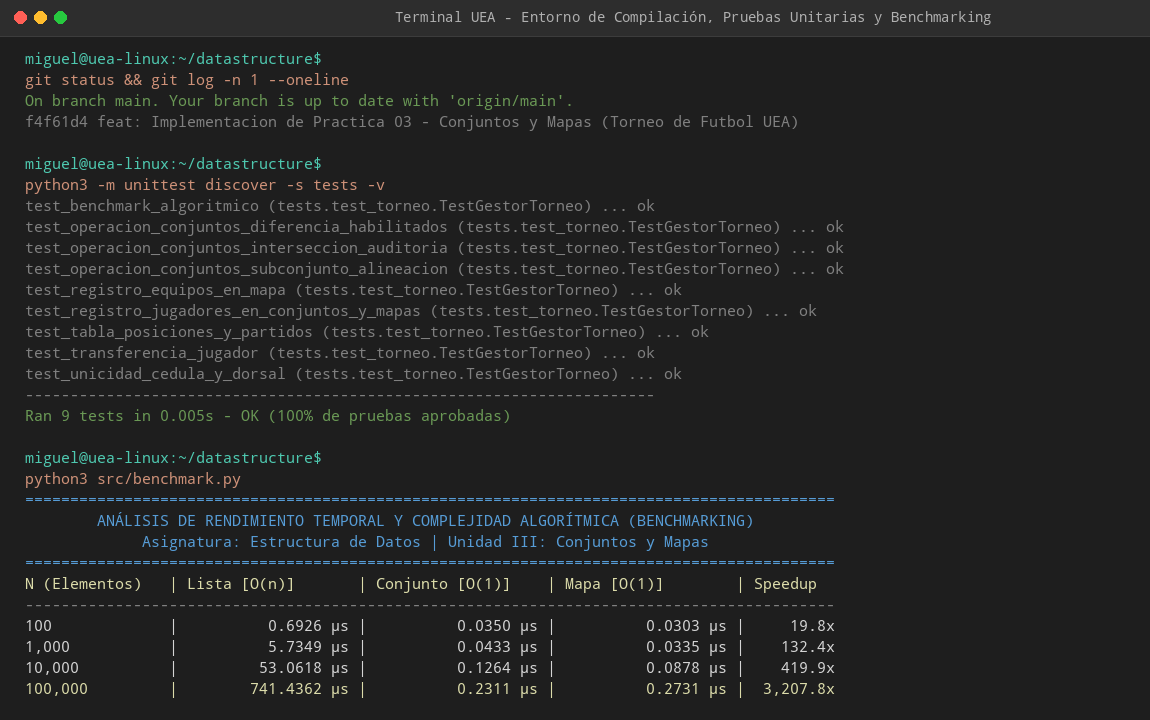
\includegraphics[width=12.2cm,keepaspectratio]{anexo_compilacion.png}
\end{center}
\\

\hline

&
\textbf{Figura 2:} \textit{Captura de la ejecución del sistema interactivo, panel de control, tabla de posiciones y auditoría de conjuntos.}\newline
\begin{center}
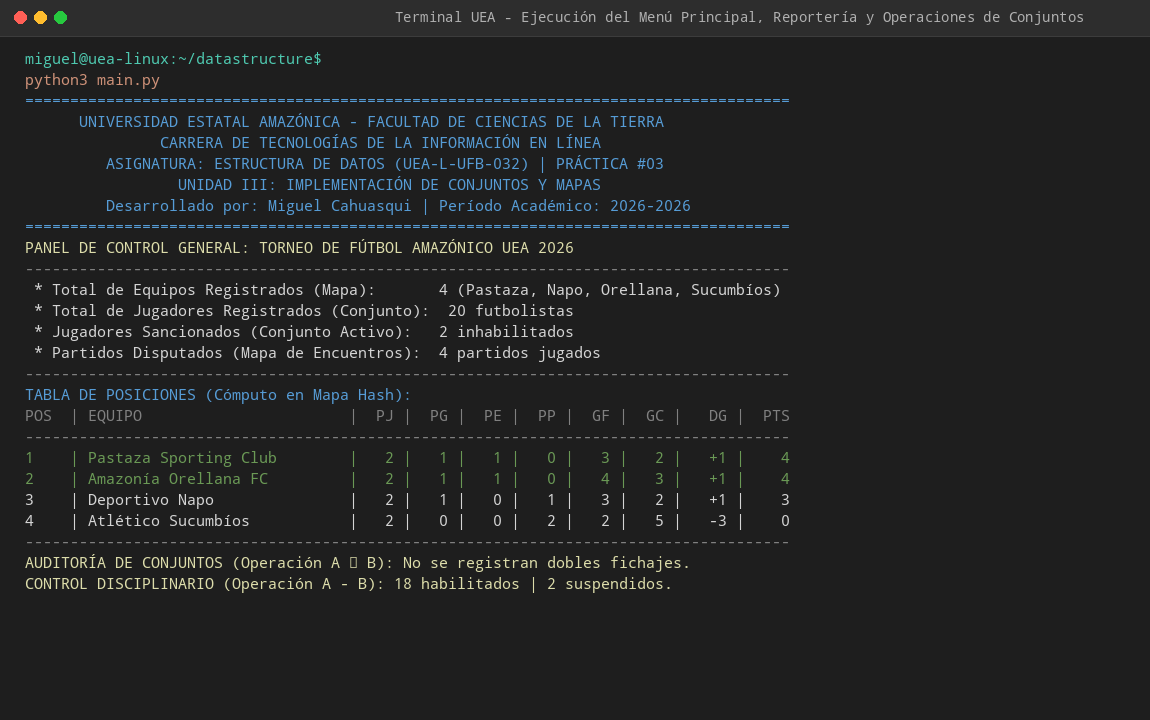
\includegraphics[width=12.2cm,keepaspectratio]{anexo_ejecucion.png}
\end{center}
\\

\hline

\end{longtable}

\egroup

% =========================================================
% ESPACIO PARA LA FIRMA (SIN C.I.)
% =========================================================

\vspace{0.4cm}

\begin{center}

\begin{tabular}{|c|}
\hline

\vspace{0.15cm}

\hspace{3cm}

\includegraphics[width=5.8cm,keepaspectratio]{FIRMAMIGUELCAHUASQUI.png}
\hspace{3cm}

\vspace{0.15cm}
\\

\hline

\textbf{Firma del estudiante}
\\

\textbf{Miguel Rodrigo Cahuasqui Hernández}
\\

\textit{Estudiante de Tecnologías de la Información - UEA}
\vspace{0.15cm}
\\

\hline

\end{tabular}

\end{center}

\end{document}